\chapter{Development}

\section{Coding style}

We use google coding style for more details see "Google C++ Style Guide" (\url{http://google-styleguide.googlecode.com/svn/trunk/cppguide.xml}) for C++ codes.

\section{How to commit changes}

\begin{itemize}

\item Commit changes in you local branch.

\begin{lstlisting}
$ git commit -a -m "My important change description."
\end{lstlisting}

\item Send your patch on code review. Use \texttt{upload.py} script (\url{https://codereview.appspot.com/static/upload.py}).

\begin{lstlisting}
$ python2.7 upload.py -m "My important change description." --rev <hash tag of last revision in remote repository>
\end{lstlisting}

For more information about usage and option of upload.py see \url{http://code.google.com/p/rietveld/wiki/UploadPyUsage}.

\item Go to \url{https://codereview.appspot.com/}, change your subject and start code review.

Click \textbf{Publish+Mail Comments} and fill the following parameters (see fig.~\ref{fig:codereview}):

\begin{itemize}
  \item Reviewers: \texttt{yulyugin@gmail.com, melges.morgen@gmail.com}
  \item CC: \texttt{mipt-smb-search-review@googlegroups.com}
  \item Description: \texttt{Description of your changes and testlog.}
\end{itemize}

\begin{figure}[htp]
  \centering
  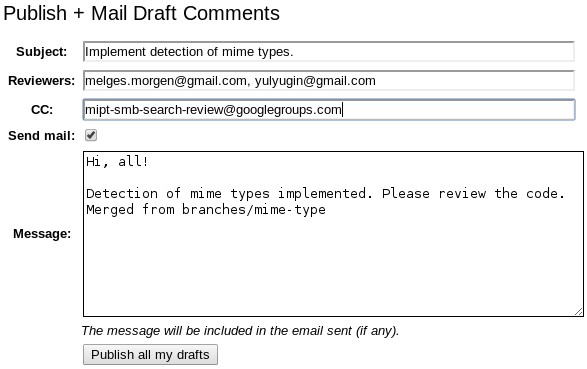
\includegraphics[width=0.6\textwidth]{./codereview.png}
  \caption{Codereview fields.}
  \label{fig:codereview}
\end{figure}

Then start codereview review by clicking \textbf{Publish all my drafts}.

\item After "LGTM" you can push your changes on the main server.

\begin{lstlisting}
git push origin master
\end{lstlisting}

\end{itemize}

\section{How to write tests}

\section{How to test coverage}

\begin{enumerate}

\item Build with TEST\_COVERAGE flag:
\begin{lstlisting}
$ make TEST_COVERAGE=yes
\end{lstlisting}

\item Run tests. For more information see section~\ref{sec:tests}

\item Go to the directory with tested file.
\begin{lstlisting}
$ cd mipt-smb-serach/spider
\end{lstlisting}

\item Test coverage with gcov programm
\begin{lstlisting}
$ gcov spider.gcda
File 'mipt-smb-search/spider/spider.cpp'
Lines executed:55.23% of 239
Creating 'spider.cpp.gcov'
\end{lstlisting}

\item You can see information about what lines and how often have been executed.
\begin{lstlisting}
$ nano spider.cpp.gcov
\end{lstlisting}

\end{enumerate}

\section{Web interface module development}

First of all you should prepare your workspace and install nesessary environment.

For developing you need:

\begin{enumerate}

\item JDK 1.6 or higher.
You can install JDK using the following commands:

For Ubuntu/Debian users:

\begin{lstlisting}
sudo apt-get install openjdk-7-jdk openjdk-7-jre
\end{lstlisting}

For OpenSUSE users:

\begin{lstlisting}
sudo zypper install java-1_7_0-openjdk jdk
\end{lstlisting}

For Arch Linux users:

\begin{lstlisting}
sudo pacman -S  jdk7-openjdk  jre7-openjdk
\end{lstlisting}

You can also download Oracle Java and install it.

\item Eclipse with GWT plugin.

More information about Eclipse set up you can find on the following web-site \url{https://developers.google.com/web-toolkit/usingeclipse}.

\item Application server (we will use Glassfish OSE).

\end{enumerate}

\subsection{System Requirements}

For comfortable developing and debugging you will need at least 2 GB of RAM and a processor Intel Core i3 or equivalent. Development of the face module is theoretically possible under Windows, but this option will not be considered.

Will agree that our user calls ``melges'', his home directory is located at /home/melges and his custom executable files are stored in ~/bin.

\section{Usefull commands for immediate work with data base.}

\begin{itemize}

\item To connect data base use following command:

\begin{lstlisting}
$ mysql db_name -u db_user -p -h db_server
\end{lstlisting}

Then enter database password.

\item To detect last element in database use following command:

\begin{lstlisting}
mysql> SELECT * FROM mss_files ORDER BY id DESC LIMIT 1;
\end{lstlisting}

\end{itemize}

\section{Qt-Creator settings}

\section{Build settings}\label{sec:qt-build}

When you open Qt-Creator at first you can see window like fig.~\ref{fig:qt-creator-config-main}. Clear "Shadow build".

\begin{figure}[htp]
  \centering
  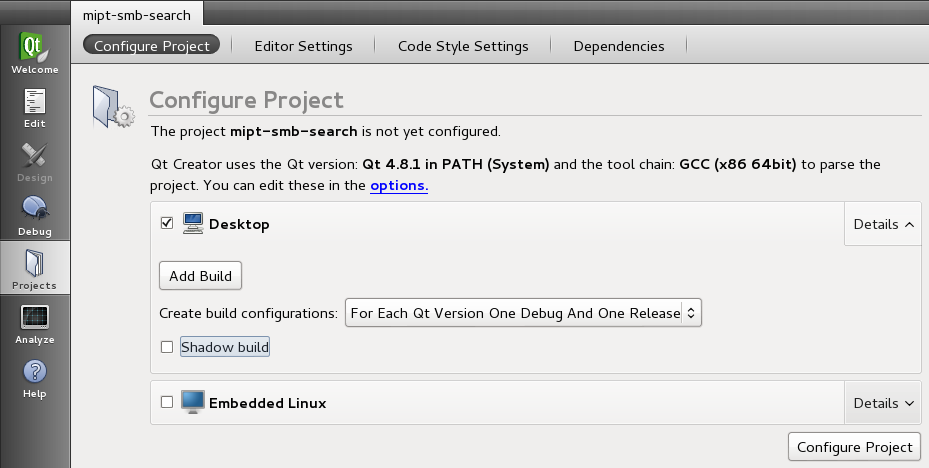
\includegraphics[width=0.8\textwidth]{./qt-creator-config-main.png}
  \caption{Qt-Creator settings main.}
  \label{fig:qt-creator-config-main}
\end{figure}

Release settings should look like fig~\ref{fig:qt-creator-config-release}. Debug settings should look like fig~\ref{fig:qt-creator-config-debug}.

\begin{figure}[htp]
  \centering
  \subfigure[]{
    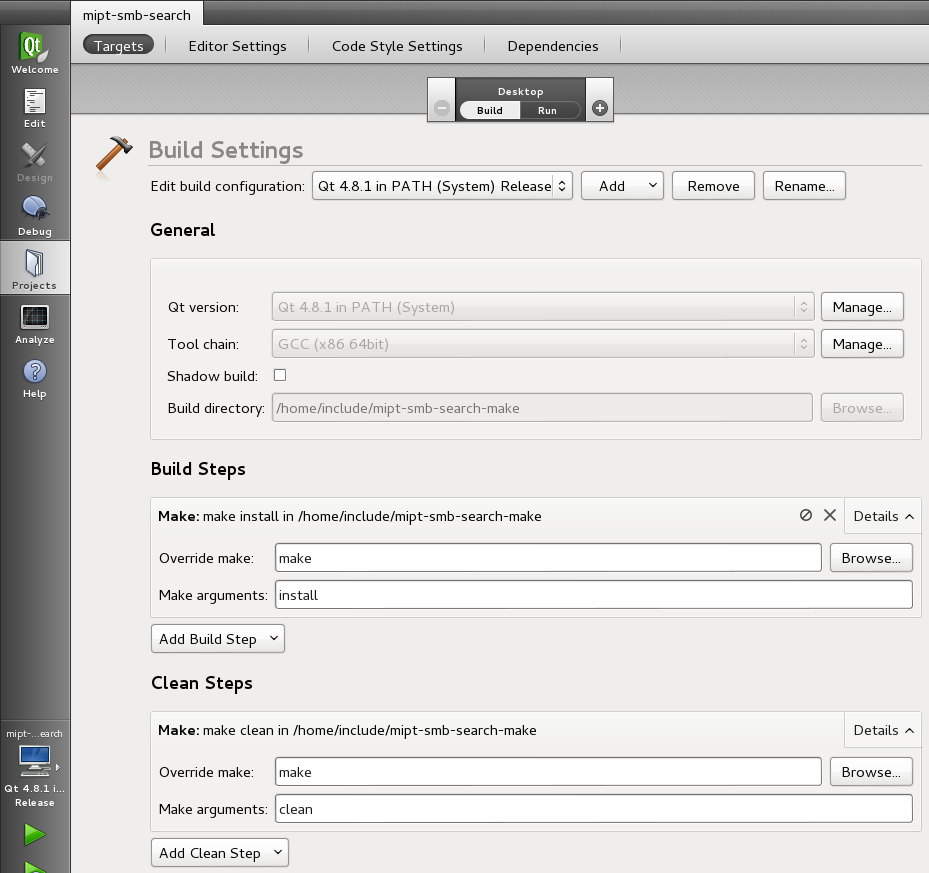
\includegraphics[width=0.8\textwidth]{./qt-creator-config-build-release.png}
    \label{fig:qt-creator-config-release}
  }
  \subfigure[]{
    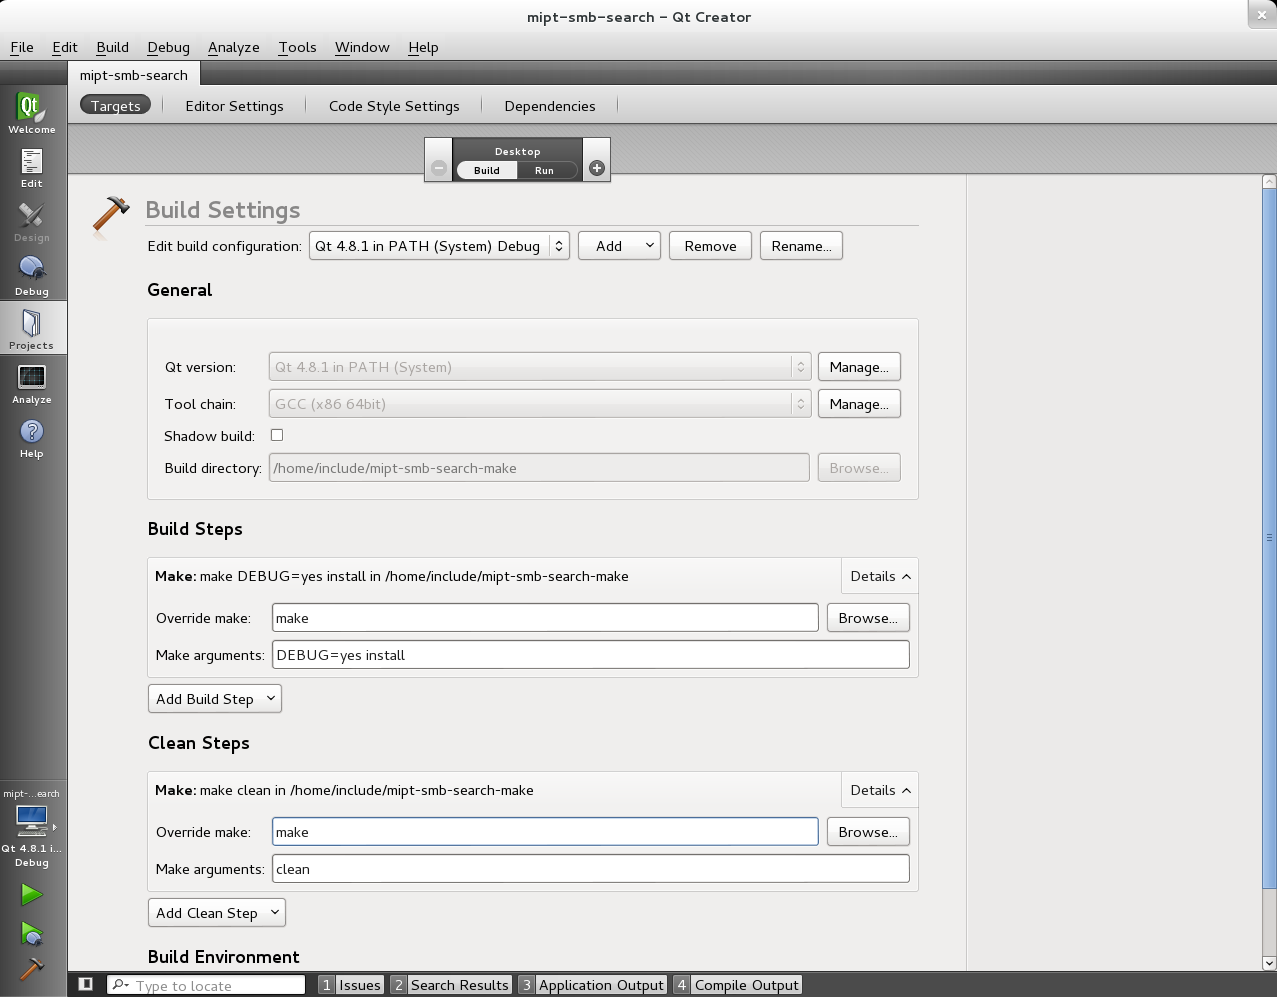
\includegraphics[width=0.8\textwidth]{./qt-creator-config-build-debug.png}
    \label{fig:qt-creator-config-debug}
  }
  \caption{Build settings for Qt-Creator: \subref{fig:qt-creator-config-release} for release build, \subref{fig:qt-creator-config-debug} for debug build.}
\end{figure}

\section{Run settings}

This is an example of Qt-Creator settings to run fulltest. These settings should be done after build settings (look at section~\ref{sec:qt-build} for more details).

\begin{enumerate}
  \item First of all you should choose path to executable file. In our example it's situated in \%{buildDir}/build/debug/tests/bin/fulltest
  \item Then add path to working directory. Fulltest should be executed from directory where it's situated. In our example it's situated in \%{buildDir}/build/debug/tests/bin
  \item You should set LD\_LIBRARY\_PATH variable to detect new shared libraries which created in our project. You should add path to lib and tests/lib folder. LD\_LIBRARY\_PATH should contain full path to this folder.
\end{enumerate}

The result of these settings could be shown in fig.~\ref{fig:qt-creator-config-run}

\begin{figure}[ht]
  \centering
  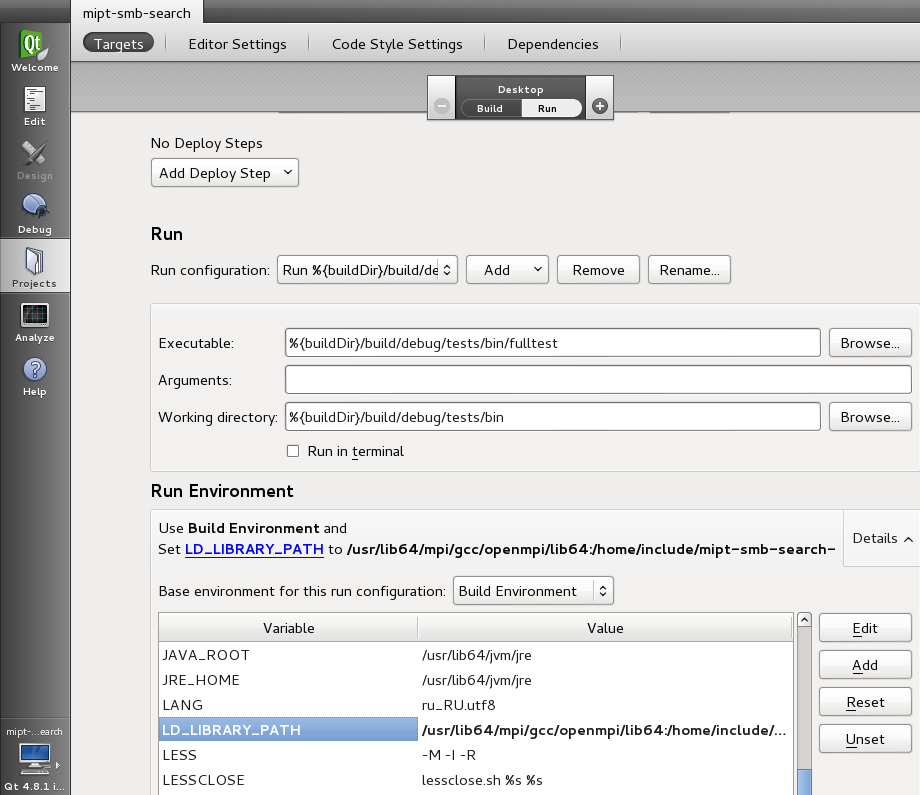
\includegraphics[width=0.8\textwidth]{./qt-creator-config-run.png}
  \caption{Qt-Creator settings to run.}
  \label{fig:qt-creator-config-run}
\end{figure}

You can configure run settings for each executable file based on this algorithm.

\printindex

\end{document}
